\newpage		
	\section{Домашнее задание 3}
		\subsection{1}	
		A)\\
		\begin{center}
			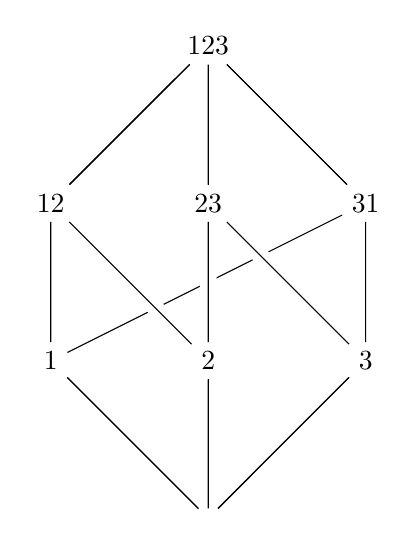
\begin{tikzpicture}
				\node (max) at (0,4) {$123$};
				
				\node (a) at (-2,2) {$12$};
				\node (b) at (0,2) {$23$};
				\node (c) at (2,2) {$31$};
				
				\node (d) at (-2,0) {$1$};
				\node (e) at (0,0) {$2$};
				\node (f) at (2,0) {$3$};
				
				\node (min) at (0,-2) {$\varnothing$};
				
				\draw (min) -- (d) -- (a) -- (max);
				\draw (min) -- (d) -- (c) -- (max);
				\draw (min) -- (e) -- (a) -- (max);
				\draw (min) -- (e) -- (b) -- (max);
				\draw (min) -- (f) -- (b) -- (max);
				\draw (min) -- (f) -- (c) -- (max);
				
				\draw[preaction={draw=white, -,line width=6pt}] (a) -- (e) -- (b) -- (f);
			\end{tikzpicture}
		\end{center}
		B)\\
		\begin{center}
			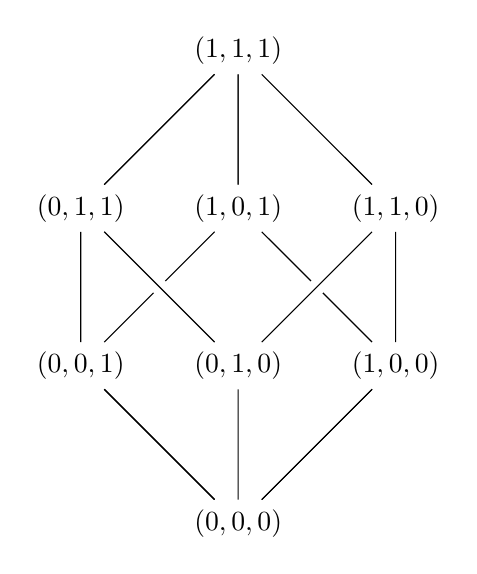
\begin{tikzpicture}
				\node (max) at (0,4) {$(1,1,1)$};
				
				\node (a) at (-2,2) {$(0,1,1)$};
				\node (b) at (0,2) {$(1,0,1)$};
				\node (c) at (2,2) {$(1,1,0)$};
				
				\node (d) at (-2,0) {$(0,0,1)$};
				\node (e) at (0,0) {$(0,1,0)$};
				\node (f) at (2,0) {$(1,0,0)$};
				
				\node (min) at (0,-2) {$(0,0,0)$};
				
				\draw (min) -- (d) -- (a) -- (max);
				\draw (min) -- (d) -- (b) -- (max);
				\draw (min) -- (e) -- (a) -- (max);
				\draw (min) -- (f) -- (b) -- (max);
				\draw (min) -- (f) -- (c) -- (max);
				\draw[preaction={draw=white, -,line width=6pt}] (a) -- (e) -- (c);
			\end{tikzpicture}
		\end{center}
		\newpage
		C)\\
		Делители числа $30$: $1,\: 2,\: 3,\: 5,\: 6,\: 10,\: 15,\: 30$\\
		Пусть множества делителей это:\\
		\begin{gather*}
		A_{30} \: = \: \{ 1,\: 2,\: 3,\: 5,\: 6,\: 10,\: 15,\: 30 \}\\
		A_{15} \: = \: \{ 1,\: 3,\: 5,\: 15 \}\\
		A_{10} \: = \: \{ 1,\: 2,\: 5,\: 10\}\\
		A_{6} \: = \: \{ 1,\: 2,\: 3,\: 6\}\\
		A_{5} \: = \: \{ 1,\: 5 \}\\
		A_{3} \: = \: \{ 1,\: 3 \}\\
		A_{2} \: = \: \{ 1,\: 2 \}\\
		A_{1} \: = \: \{ 1 \}
		\end{gather*}
		Тогда
		\begin{center}
			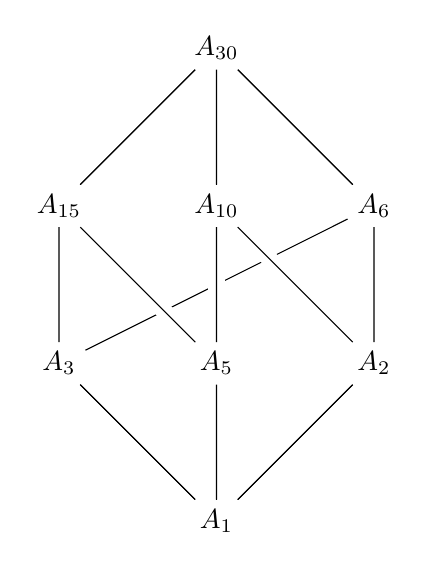
\begin{tikzpicture}
				\node (max) at (0,4) {$A_{30}$};
				
				\node (a) at (-2,2) {$A_{15}$};
				\node (b) at (0,2) {$A_{10}$};
				\node (c) at (2,2) {$A_{6}$};
				
				\node (d) at (-2,0) {$A_{3}$};
				\node (e) at (0,0) {$A_{5}$};
				\node (f) at (2,0) {$A_{2}$};
				
				\node (min) at (0,-2) {$A_{1}$};
				
				\draw (min) -- (d) -- (a) -- (max);
				\draw (min) -- (d) -- (c) -- (max);
				\draw (min) -- (e) -- (a) -- (max);
				\draw (min) -- (e) -- (b) -- (max);
				\draw (min) -- (f) -- (b) -- (max);
				\draw (min) -- (f) -- (c) -- (max);
				\draw[preaction={draw=white, -,line width=6pt}] (a) -- (e) -- (b) -- (f);
			\end{tikzpicture}
		\end{center}
		
		\subsection{2}
		1)\\
		Сопоставим каждому вектору $a$ число $N_a = a_1*2^{n-1} + a_2*2^{n-2} + ... + a_n*2^0$. Нетрудно видеть, что тогда $a \preceq_1 b \: \Leftrightarrow \: N_a \leq N_b$, при этом "$\leq$" является отношением линейного порядка, откуда  "$\preceq_1$" также является отношением линейного порядка, т.к. для всех $a,b : a \ne b \Rightarrow N_a \ne N_b$, т.к. коэффициэнты не превосходят 1, откуда пусть первое различие в $k$-том элементе, тогда тот вектор, у которого 1, будет больше второго вектора вне зависимости от последующих коэффициэнтов.\\
		2)\\
		Нетрудно видеть, что $a \preceq_3 b \: \Leftrightarrow \: a \preceq_1 b$ (можем аналогично сопоставлять вектору число, при этом если 2 вектора отличаются впервые в $k$-том элементе, тогда тот вектор, у которого 1, будет больше второго вектора в "$\preceq_3$" по определению и в "$\preceq_1$", т.к. $2^k > 2^{k-1} + 2^{k-2} + ... + 1$.
		
		\newpage
		\subsection{3}
		A)\\
		Рассмотрим все возможные способы представить 4 в виде суммы неупорядоченных слагаемых.\\
		Они следующие:
		\begin{gather*}
			\begin{matrix}
				1. & 1 + 1 + 1 + 1\\
				2. & 2 + 1 + 1\\
				3. & 2 + 2\\
				4. & 3 + 1\\
				5. & 4
			\end{matrix}
		\end{gather*}
		Заметим, что выше указаны все возможные варианты мощностей классов эквивалентности.\\
		Посчитаем, столько отношений эквивалентности для каждого варианта:
		\begin{gather*}
			\begin{matrix}
				1. & 1\\
				2. & \frac{4*3}{2}\\
				3. & \frac{4*3}{2*2}\\
				4. & 4\\
				5. & 1
			\end{matrix}
		\end{gather*}
		Откуда всего разных отношений эквивалетности $1 + 6 + 3 + 4 + 1 = 15$.
		\\ \\
		B)\\
		Докажем, что у каждого линейного отношения конечного множества есть "минимальный" элемент $x$, то есть такой, что $x \leq y$ для $\forall y$. Докажем по индукции по $n$ где мощность множества = $n$. База - $n = 1$ - очевидна. Переход : пусть для любого множества мощности $n$. Тогда рассмотрим множество мощности $n+1$ и линейное отношение. Рассмотрим любые 2 различных элемента (они есть т.к. n > 1), и рассмотрим среди них "большее". "Удалим" его из множества и линейного отношения. Для оставшегося множества и линейного отношения есть минимальное, нетрудно  видеть, что минимальное меньше чем удалённый элемент из транзитивности.\\
		При этом среди множества без минимального элемента есть также минимальный элемент, в множестве без 2х минимальных - ещё 1 и тд. Пронумераем минимальные элементы от 1 до $n$. Тогда для всех элементов $a_i$ и $a_j$, что $i \leq j$ верно, что $a_i \leq a_j$. Таким образом каждое линейное отношение задаётся нумерацией элементов от 1 до $n$, таким образом линейных отношений $n!$. 
		Ответ: $4! = 24$.